\lecture{14}{20 Nov.}{}

\section{The Algorithmic Local Lemma}\label{sec:algorithmic-lll}

\subsection{Finding the Coloring}\label{sec:alll-problem}

Let \(H\) be a \(k\)-uniform hypergraph with edges \(F_{1}, \ldots, F_{m}\), each meeting few others. \autoref{prop:property-B-lll} shows that \(H\) has a \(2\)-coloring without monochromatic edges (call such a coloring \vocab{good}), but the proof only shows that a random coloring is good with \emph{positive} probability. It does not tell us how to \emph{find} a good coloring. The question of this section is whether a good coloring can be found quickly, i.e.\ in time polynomial in \(m\).

\emph{The naive algorithm.} The obvious idea is to turn the proof into an algorithm: pick a uniformly random coloring, check whether it is good, and if not, discard it and try again with a fresh random coloring. Write
\[
    p_{\mathrm{good}} \coloneqq \mathbb{P}(\text{a uniformly random coloring is good}) = \mathbb{P}\Bigl( \bigcap_{i=1}^{m} A_{i}^{c} \Bigr) > 0 ,
\]
where \(A_{i} \coloneqq \{ F_{i} \text{ is monochromatic} \}\) as in the proof of \autoref{prop:property-B-lll} (there \(p = \mathbb{P}(A_{i}) = 2^{1-k}\) is the probability of a single bad event, which is different). The trials are independent, each succeeding with probability \(p_{\mathrm{good}}\), so the number of trials until the first good coloring is \(\mathrm{Geom}(p_{\mathrm{good}})\), with mean \(\frac{1}{p_{\mathrm{good}}}\). So this algorithm is fast exactly when \(p_{\mathrm{good}}\) is not too small.

\emph{Why the local lemma gives a tiny \(p_{\mathrm{good}}\).} To apply \thmref{thm:lll-general} one needs weights \(x_{1}, \ldots, x_{m} \in [0,1)\) satisfying \eqref{eq:lll-general-condition}, i.e.\ \(\mathbb{P}(A_{i}) \le x_{i} \prod_{j : (i,j) \in E(\Gamma)} (1 - x_{j}) \le x_{i}\); so every such choice has \(x_{i} \ge \mathbb{P}(A_{i}) = 2^{1-k}\). Hence the lower bound on \(p_{\mathrm{good}}\) that \thmref{thm:lll-general} gives is at most
\[
    \prod_{i=1}^{m} (1 - x_{i}) \le \bigl( 1 - 2^{1-k} \bigr)^{m} \le e^{-m 2^{1-k}} ,
\]
which is exponentially small in \(m\) (for fixed \(k\)). So from the local lemma alone we can only promise about \(e^{m 2^{1-k}}\) trials, exponential in \(m\). This is not just a weakness of the bound. Suppose \(F_{1}, \ldots, F_{m}\) are pairwise disjoint (so each edge meets no other edge, and the hypothesis of \autoref{prop:property-B-lll} certainly holds). Then:
\begin{itemize}
    \item \emph{One edge.} \(F_{i}\) is monochromatic iff its \(k\) vertices are all \(0\) or all \(1\), so \(\mathbb{P}(A_{i}) = 2 \cdot 2^{-k} = 2^{1-k}\) and \(\mathbb{P}(A_{i}^{c}) = 1 - 2^{1-k}\).
    \item \emph{Independence.} \(A_{i}\) is determined by the colors of the vertices of \(F_{i}\). Since the sets \(F_{1}, \ldots, F_{m}\) are pairwise disjoint and the vertices are colored independently, \(A_{1}, \ldots, A_{m}\) are determined by disjoint groups of independent colors, so they are mutually independent, and hence so are \(A_{1}^{c}, \ldots, A_{m}^{c}\) (\autoref{rmk:mutual-indep-complements}).
    \item \emph{Multiplying.} Therefore
    \[
        p_{\mathrm{good}} = \mathbb{P}\Bigl( \bigcap_{i=1}^{m} A_{i}^{c} \Bigr) = \prod_{i=1}^{m} \mathbb{P}(A_{i}^{c}) = \bigl( 1 - 2^{1-k} \bigr)^{m} .
    \]
\end{itemize}
So here \(p_{\mathrm{good}}\) equals the bound above exactly, and the naive algorithm needs \(\frac{1}{p_{\mathrm{good}}} = (1 - 2^{1-k})^{-m} \ge e^{m 2^{1-k}}\) trials on average, which is exponential in \(m\).

\emph{The fix.} In the disjoint example the naive algorithm is wasteful: when only \(F_{3}\) is monochromatic, it throws away the whole coloring, although recoloring the \(k\) vertices of \(F_{3}\) alone would do. The algorithms below keep the coloring and repair it locally, recoloring only the vertices of a monochromatic edge. This turns out to be fast whenever each edge meets few others.

\begin{theorem}[Beck, 1991]\label{thm:beck}
    There is \(c > 0\) such that if every edge of a \(k\)-uniform hypergraph \(H\) intersects at most \(2^{ck}\) edges, then a \(2\)-coloring of \(H\) without monochromatic edges can be found in polynomial time.
\end{theorem}

We do not prove \autoref{thm:beck}, since the following theorem improves it.

\begin{theorem}[Moser--Tardos]\label{thm:moser-tardos}
    Let \(H\) be a \(k\)-uniform hypergraph with \(m\) edges in which every edge intersects at most \(2^{k-4}\) edges (itself included). Then there is a randomized algorithm that finds a \(2\)-coloring of \(H\) without monochromatic edges in expected time \(O(m \log m)\).
\end{theorem}

Up to the constant in the exponent, this is the condition of \autoref{prop:property-B-lll}, which needs \(\le \frac{2^{k-1}}{e} - 1\) other edges. The algorithm colors the vertices at random, and while some edge is monochromatic it recolors the vertices of that edge at random. Recoloring an edge can create new monochromatic edges, but only among the edges meeting it, and these are repaired first.

\subsection{The Algorithm}\label{sec:alll-algorithm}

\emph{Setup.} Fix an ordering \(E(H) = \{ F_{1}, \ldots, F_{m} \}\) of the edges once and for all; the \vocab{index} of \(F_{i}\) is \(i\). The algorithm always repairs the monochromatic edge of smallest index first, so the ordering only serves to break ties. The two colors are \(0\) and \(1\). For an edge \(F\), let \(N(F)\) be the set of edges meeting \(F\), \(F\) itself included:
\[
    N(F) \coloneqq \{ G \in E(H) : G \cap F \ne \varnothing \},
    \qquad \abs{N(F)} \le 2^{k-4}
\]
by the hypothesis of \autoref{thm:moser-tardos}.

\emph{The two procedures.} The algorithm consists of a main procedure \textsc{LLL-Painter} (\autoref{alg:lll-painter}) and a recursive procedure \textsc{LLL-Repainter} (\autoref{alg:lll-repainter}). \textsc{LLL-Painter} colors \(V(H)\) at random and, as long as some edge is monochromatic, hands the one of smallest index to \textsc{LLL-Repainter}. \textsc{LLL-Repainter}\((H, F, c)\), where \(c\) is the current coloring and \(F\) an edge monochromatic in \(c\), recolors the vertices of \(F\) at random and then, as long as some edge of \(N(F)\) is monochromatic, calls itself on the one of smallest index. Each execution of \textsc{LLL-Repainter}\((H, F, c)\) is a \vocab{call on \(F\)}, and we number the calls \(1, 2, 3, \ldots\) in the order in which they start. A call made by \textsc{LLL-Painter} is a \vocab{top-level call}. The calls form the \vocab{coloring tree} (\autoref{fig:coloring-tree} below): its root is \textsc{LLL-Painter}, and the children of a call are the calls it makes, in order.

\emph{The log.} Besides the coloring, the algorithm writes a binary string \(\mathrm{Log}\). It does not influence the run; it records which edges are recolored, in which order, so that the analysis can reconstruct the run from it (\autoref{lem:log-length}). It uses the following notation.

\begin{notation}\label{nota:log}
    \leavevmode
    \begin{itemize}
        \item \(\mathrm{Log}\) is a global binary string, initially empty, and \(+\) is concatenation of strings; \(\texttt{1}\) and \(\texttt{0}\) are single bits.
        \item \(\operatorname{col}(F) \in \{0, 1\}\), for a monochromatic edge \(F\), is the common color of the vertices of \(F\) (\(1\) bit).
        \item \(\operatorname{index}(i)\), for \(1 \le i \le m\), is the number \(i - 1 \in \{0, \ldots, m-1\}\) written in binary with \(\lceil \log_{2} m \rceil\) bits. It names \(F_{i}\) among all \(m\) edges.
        \item \(\operatorname{relindex}(G, F)\), the \emph{relative index} of \(G \in N(F)\), is defined as follows: list \(N(F) = \{ G_{0}, G_{1}, \ldots \}\) in increasing order of index; then \(\operatorname{relindex}(G, F) \coloneqq j\) where \(G = G_{j}\), written in binary with \(k - 4\) bits, which is possible as \(j < \abs{N(F)} \le 2^{k-4}\). It names \(G\) among the edges meeting \(F\) only, and together with \(F\) determines \(G\).
    \end{itemize}
\end{notation}

Just before a call on an edge \(G\) starts, its \vocab{record} is appended to \(\mathrm{Log}\): the bit \(\texttt{1}\), then the name of \(G\), then \(\operatorname{col}(G)\). For a top-level call on \(G = F_{i}\) the name is \(\operatorname{index}(i)\), so the record has \(\lceil \log_{2} m \rceil + 2\) bits. For a call on \(G\) made inside a call on \(F\), the edge \(G\) meets \(F\), so the name \(\operatorname{relindex}(G, F)\) suffices, and the record has \(1 + (k - 4) + 1 = k - 2\) bits; this is what keeps \(\mathrm{Log}\) short. When a call returns, the bit \(\texttt{0}\) is appended.

\begin{algorithm}[H]
    \SetFuncSty{textsc}
    \SetKwFunction{Repainter}{LLL-Repainter}
    \caption{\textsc{LLL-Painter}\((H)\)}\label{alg:lll-painter}
    \KwIn{a \(k\)-uniform hypergraph \(H\) with edges \(F_{1}, \ldots, F_{m}\)}
    \KwOut{a \(2\)-coloring \(c\) of \(V(H)\) without monochromatic edges}
    \(c \gets\) a uniformly random coloring \(V(H) \to \{0, 1\}\)\;
    \(\mathrm{Log} \gets\) the empty string\;
    \While{some edge is monochromatic in \(c\)}{
        \(i \gets\) the smallest index such that \(F_{i}\) is monochromatic\;
        \(\mathrm{Log} \gets \mathrm{Log} + \texttt{1} + \operatorname{index}(i) + \operatorname{col}(F_{i})\) \tcp*{\(\lceil \log_{2} m \rceil + 2\) bits}
        \(c \gets\) \Repainter{\(H, F_{i}, c\)}\;
    }
    \Return{\(c\)}
\end{algorithm}

\begin{algorithm}[H]
    \SetFuncSty{textsc}
    \SetKwFunction{Repainter}{LLL-Repainter}
    \caption{\textsc{LLL-Repainter}\((H, F, c)\)}\label{alg:lll-repainter}
    \KwIn{a \(k\)-uniform hypergraph \(H\), an edge \(F\) monochromatic in \(c\), a coloring \(c\)}
    \KwOut{the updated coloring \(c\), in which no edge of \(N(F)\) is monochromatic}
    \ForEach{\(v \in F\)}{
        \(c(v) \gets\) a uniformly random color in \(\{0, 1\}\), independent of everything before\;
    }
    \While{some \(G \in N(F)\) is monochromatic in \(c\)}{
        \(G \gets\) the one with the smallest index\;
        \(\mathrm{Log} \gets \mathrm{Log} + \texttt{1} + \operatorname{relindex}(G, F) + \operatorname{col}(G)\) \tcp*{\(k - 2\) bits}
        \(c \gets\) \Repainter{\(H, G, c\)} \tcp*{the updated coloring}
    }
    \(\mathrm{Log} \gets \mathrm{Log} + \texttt{0}\) \tcp*{\(1\) bit}
    \Return{\(c\)} \tcp*{the coloring after all the recolorings above}
\end{algorithm}

For example, if a top-level call on \(F_{3}\) makes a single call, on some \(G \in N(F_{3})\), the two calls write
\[
    \underbrace{\texttt{1} + \operatorname{index}(3) + \operatorname{col}(F_{3})}_{\text{record of the call on } F_{3}}
    + \underbrace{\texttt{1} + \operatorname{relindex}(G, F_{3}) + \operatorname{col}(G)}_{\text{record of the call on } G}
    + \underbrace{\texttt{0}}_{G \text{ returns}} + \underbrace{\texttt{0}}_{F_{3} \text{ returns}} .
\]

\emph{Termination.} Nothing so far guarantees that a call returns, or that \textsc{LLL-Painter} stops: the random recolorings could, for instance, keep making the same edges monochromatic forever. We show in the proof of \autoref{thm:moser-tardos} that this happens with probability \(0\). Until then, statements about a call assume that it returns, as in \autoref{lem:repainter-returns}.

\begin{lemma}\label{lem:repainter-returns}
    Suppose \textsc{LLL-Repainter}\((H, F, c)\) returns the coloring \(c'\). Then
    \begin{enumerate}[(i)]
        \item no edge of \(N(F)\) is monochromatic in \(c'\);
        \item every edge \(G\) monochromatic in \(c'\) is monochromatic in \(c\), and \(c' = c\) on \(G\).
    \end{enumerate}
\end{lemma}

\begin{proof}
    (i) is the exit condition of the while loop of \autoref{alg:lll-repainter}.

    For (ii), we induct on the total number \(n\) of calls in the subtree of the coloring tree rooted at this call, i.e.\ the call itself together with all calls made during it (its children, their children, and so on); \(n\) is finite because the call returned. Let \(r \ge 0\) be the number of children of the call on \(F\), let \(F^{(1)}, \ldots, F^{(r)}\) be their edges, and follow the coloring during the call (\autoref{fig:repainter-colorings}):
    \begin{itemize}
        \item \(c_{0}\) is the coloring right after the vertices of \(F\) are recolored, so \(c_{0} = c\) outside \(F\);
        \item \(c_{s}\) is the coloring returned by the \(s\)-th child, which is the call on \(F^{(s)}\) with input \(c_{s-1}\); so \(c_{r} = c'\).
    \end{itemize}
    In the base case \(n = 1\) the call makes no call, so \(r = 0\) and \(c' = c_{0}\); the argument below covers this case too.
    Let \(G\) be monochromatic in \(c' = c_{r}\). The subtree of the \(s\)-th child has \(< n\) calls, so the induction hypothesis applies to it, with input \(c_{s-1}\) and output \(c_{s}\): if \(G\) is monochromatic in \(c_{s}\), then it is monochromatic in \(c_{s-1}\) and \(c_{s-1} = c_{s}\) on \(G\). Applying this for \(s = r, r-1, \ldots, 1\), \(G\) is monochromatic in \(c_{0}\) and \(c_{0} = c'\) on \(G\). By (i), \(G \notin N(F)\), i.e.\ \(G \cap F = \varnothing\), so \(c_{0} = c\) on \(G\). Hence \(c = c_{0} = c'\) on \(G\), and \(G\) is monochromatic in \(c\).
\end{proof}

\begin{figure}[H]
    \centering
    \begin{tikzpicture}[every node/.style={font=\small}]
        \node (root) at (3.5, 0) {call on \(F\)};
        \foreach \x/\lab/\nm in {1/{F^{(1)}}/k1, 3.5/{F^{(2)}}/k2, 7/{F^{(r)}}/kr} {
            \node (\nm) at (\x, -1.3) {\(\lab\)};
            \draw (root) -- (\nm);
            \draw (\x, -1.55) -- (\x - 0.6, -2.6) -- (\x + 0.6, -2.6) -- cycle;
        }
        \node at (5.25, -1.3) {\(\cdots\)};
        \node[font=\footnotesize, align=center] at (-1.4, -1.9) {children's\\ subtrees \(\to\)};

        % the colorings during the call
        \node (c)  at (-2.3, -3.4) {\(c\)};
        \node (c0) at (-0.2, -3.4) {\(c_{0}\)};
        \node (c1) at (2.25, -3.4) {\(c_{1}\)};
        \node (c2) at (4.75, -3.4) {\(c_{2}\)};
        \node (cr1) at (5.9, -3.4) {\(c_{r-1}\)};
        \node (cr) at (8.3, -3.4) {\(c_{r} = c'\)};
        \draw[-Stealth] (c) -- node[above, font=\footnotesize] {recolor \(F\)} (c0);
        \draw[-Stealth] (c0) -- node[below, font=\footnotesize] {child \(1\)} (c1);
        \draw[-Stealth] (c1) -- node[below, font=\footnotesize] {child \(2\)} (c2);
        \draw[dotted] (c2) -- (cr1);
        \draw[-Stealth] (cr1) -- node[below, font=\footnotesize] {child \(r\)} (cr);
    \end{tikzpicture}
    \caption{The colorings during a call on \(F\) (\autoref{lem:repainter-returns}). The call first recolors \(F\), turning \(c\) into \(c_{0}\). Then its \(s\)-th child, on \(F^{(s)}\), together with all calls below it, turns \(c_{s-1}\) into \(c_{s}\); the induction hypothesis is applied to these \(r\) smaller subtrees.}
    \label{fig:repainter-colorings}
\end{figure}

By (ii) of \autoref{lem:repainter-returns}, read contrapositively, a call never makes an edge monochromatic that was not monochromatic when the call started. So once an edge has been repaired, later calls at the same level of the coloring tree cannot break it again, and no edge is repaired twice at the same level.

\begin{corollary}\label{cor:top-level-once}
    In every run of \textsc{LLL-Painter}, the following hold.
    \begin{enumerate}[(i)]
        \item The top-level calls are on pairwise distinct edges. In particular, \textsc{LLL-Painter} makes at most \(m\) top-level calls.
        \item For every call on an edge \(F\), its children are calls on pairwise distinct edges of \(N(F)\). In particular, every call has at most \(\abs{N(F)} \le 2^{k-4}\) children.
    \end{enumerate}
\end{corollary}

\begin{proof}
    (i) Take two top-level calls, an earlier one on \(F_{i}\) and a later one on \(F_{j}\). \textsc{LLL-Painter} starts a call only after the previous one has returned, so the call on \(F_{i}\) and every top-level call between the two have returned.
    \begin{itemize}
        \item When the call on \(F_{i}\) returns, \(F_{i}\) is not monochromatic, by (i) of \autoref{lem:repainter-returns} and \(F_{i} \in N(F_{i})\).
        \item Each top-level call in between keeps \(F_{i}\) non-monochromatic, by (ii) of \autoref{lem:repainter-returns}.
        \item So \(F_{i}\) is not monochromatic when the call on \(F_{j}\) starts, whereas \(F_{j}\) is, since calls are made only on monochromatic edges.
    \end{itemize}
    Hence \(F_{i} \ne F_{j}\). As \(H\) has \(m\) edges, there are at most \(m\) top-level calls.

    (ii) The children of a call on \(F\) are made by its while loop, one after another, each after the previous one has returned, and \(F\) is recolored only before the loop starts. The edges of the children lie in \(N(F)\) by the loop condition, and the argument of (i), with the call on \(F\) in place of \textsc{LLL-Painter}, shows that they are pairwise distinct.
\end{proof}

\begin{figure}[H]
    \centering
    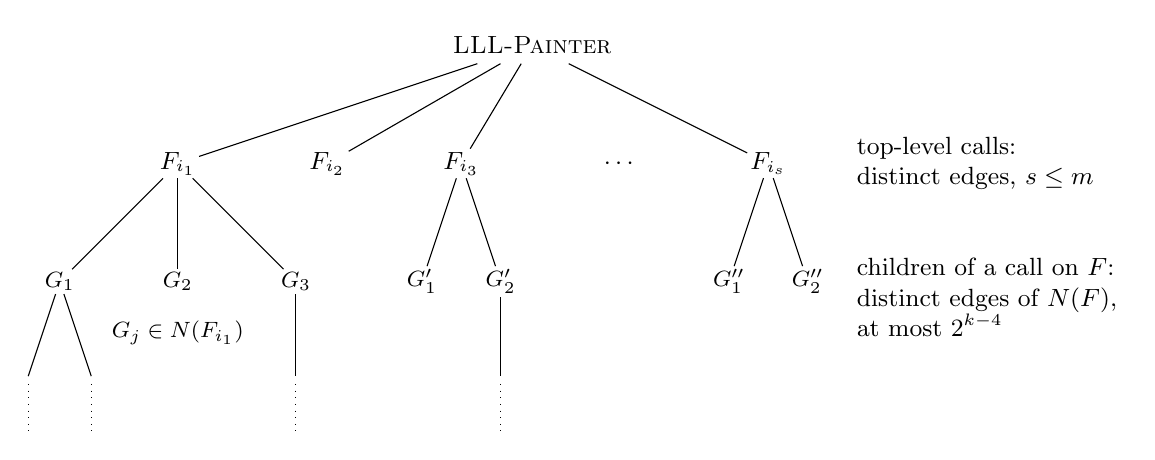
\begin{tikzpicture}[
            every node/.style={font=\small},
            level1/.style={inner sep=1pt},
            sub/.style={inner sep=1pt, font=\footnotesize},
        ]
        \node (r) at (0, 0) {\textsc{LLL-Painter}};

        \node[level1] (a1) at (-4.5, -1.5) {\(F_{i_{1}}\)};
        \node[level1] (a2) at (-2.6, -1.5) {\(F_{i_{2}}\)};
        \node[level1] (a3) at (-0.9, -1.5) {\(F_{i_{3}}\)};
        \node at (1.1, -1.5) {\(\cdots\)};
        \node[level1] (as) at (3.0, -1.5) {\(F_{i_{s}}\)};
        \foreach \v in {a1, a2, a3, as} \draw (r) -- (\v);

        % children of F_{i_1}: edges of N(F_{i_1})
        \node[sub] (b1) at (-6.0, -3.0) {\(G_{1}\)};
        \node[sub] (b2) at (-4.5, -3.0) {\(G_{2}\)};
        \node[sub] (b3) at (-3.0, -3.0) {\(G_{3}\)};
        \foreach \v in {b1, b2, b3} \draw (a1) -- (\v);
        \draw (b1) -- (-6.4, -4.2);
        \draw (b1) -- (-5.6, -4.2);
        \draw (b3) -- (-3.0, -4.2);
        \draw[dotted] (-6.4, -4.3) -- (-6.4, -4.9);
        \draw[dotted] (-5.6, -4.3) -- (-5.6, -4.9);
        \draw[dotted] (-3.0, -4.3) -- (-3.0, -4.9);

        % children of F_{i_3}
        \node[sub] (c1) at (-1.4, -3.0) {\(G'_{1}\)};
        \node[sub] (c2) at (-0.4, -3.0) {\(G'_{2}\)};
        \foreach \v in {c1, c2} \draw (a3) -- (\v);
        \draw (c2) -- (-0.4, -4.2);
        \draw[dotted] (-0.4, -4.3) -- (-0.4, -4.9);

        % children of F_{i_s}
        \node[sub] (d1) at (2.5, -3.0) {\(G''_{1}\)};
        \node[sub] (d2) at (3.5, -3.0) {\(G''_{2}\)};
        \foreach \v in {d1, d2} \draw (as) -- (\v);

        \node[align=left, anchor=west] at (4.0, -1.5) {top-level calls:\\ distinct edges, \(s \le m\)};
        \node[align=left, anchor=west] at (4.0, -3.2) {children of a call on \(F\):\\ distinct edges of \(N(F)\),\\ at most \(2^{k-4}\)};
        \node[font=\footnotesize] at (-4.5, -3.65) {\(G_{j} \in N(F_{i_{1}})\)};
    \end{tikzpicture}
    \caption{The coloring tree. \(F_{i_{1}}, \ldots, F_{i_{s}}\) are the edges of the top-level calls in order, and the \(G\)'s below a call are the edges of its children. By \autoref{cor:top-level-once}, the root has at most \(m\) children and every other vertex has at most \(2^{k-4}\).}
    \label{fig:coloring-tree}
\end{figure}

\emph{A faster main loop.} \autoref{alg:lll-painter} searches for the monochromatic edge of smallest index from \(F_{1}\) again in every pass of its while loop, but it suffices to search forward. Suppose a top-level call is made on \(F_{i}\), the monochromatic edge of smallest index. After it returns, \(F_{i}\) is not monochromatic by (i) of \autoref{lem:repainter-returns}, and every monochromatic edge was already monochromatic before the call by (ii) of \autoref{lem:repainter-returns}, so it has index \(> i\). Hence the next search may start at \(F_{i+1}\). \autoref{alg:lll-painter-scan} does exactly this, and with the same random colors it makes the same calls as \autoref{alg:lll-painter}.

\begin{algorithm}[H]
    \SetFuncSty{textsc}
    \SetKwFunction{Repainter}{LLL-Repainter}
    \caption{\textsc{LLL-Painter-Scan}\((H)\)}\label{alg:lll-painter-scan}
    \KwIn{a \(k\)-uniform hypergraph \(H\) with edges \(F_{1}, \ldots, F_{m}\)}
    \KwOut{a \(2\)-coloring \(c\) of \(V(H)\) without monochromatic edges}
    \(c \gets\) a uniformly random coloring \(V(H) \to \{0, 1\}\)\;
    \(\mathrm{Log} \gets\) the empty string\;
    \For{\(i = 1, \ldots, m\)}{
        \If{\(F_{i}\) is monochromatic in \(c\)}{
            \(\mathrm{Log} \gets \mathrm{Log} + \texttt{1} + \operatorname{index}(i) + \operatorname{col}(F_{i})\)\;
            \(c \gets\) \Repainter{\(H, F_{i}, c\)}\;
        }
    }
    \Return{\(c\)}
\end{algorithm}

\subsection{Analysis}\label{sec:alll-analysis}

Throughout, a \emph{call} means a call of \textsc{LLL-Repainter}, top-level or not, as in \autoref{sec:alll-algorithm}; \textsc{LLL-Painter} itself is not counted. Let
\[
    T \coloneqq \text{the total number of calls of \textsc{LLL-Repainter} during the whole run} \in \{0, 1, 2, \ldots\} \cup \{\infty\},
\]
where \(T = \infty\) if the run never stops. Note that \(T\) counts calls, not running time; the two are compared at the end of the proof of \autoref{thm:moser-tardos}. Recall that the calls are numbered \(1, 2, 3, \ldots\) in the order in which they start. For the \(s\)-th call let
\begin{itemize}
    \item \(E_{s}\) be its edge;
    \item \(\gamma_{s} \in \{0, 1\}\) be the color of \(E_{s}\) when the call starts. \(E_{s}\) is monochromatic at that moment, and \(\gamma_{s}\) is the last bit of the record of the call.
\end{itemize}
For \(t \le T\), let \(\mathrm{Log}_{t}\) be \(\mathrm{Log}\) right after the record of the \(t\)-th call is written. \autoref{fig:log-example} shows an example.

\begin{figure}[H]
    \centering
    \begin{tikzpicture}[
            every node/.style={font=\footnotesize},
            bit/.style={draw, minimum height=5mm, inner sep=2pt, anchor=west},
            call/.style={inner sep=3pt},
        ]
        % coloring tree
        \node (root) at (5.6, 3.5) {\textsc{LLL-Painter}};
        \node[call] (n1) at (1.4, 2.5) {call \(1\): \(E_{1} = F_{3}\)};
        \node[call] (n2) at (3.4, 1.6) {call \(2\): \(E_{2} = G\)};
        \node[call] (n3) at (6.4, 0.7) {call \(3\): \(E_{3} = G'\)};
        \node[call] (n4) at (11.6, 2.5) {call \(4\): \(E_{4} = F_{5}\)};
        \draw (root.south) -- (n1.north);
        \draw (root.south) -- (n4.north);
        \draw (n1.south east) -- (n2.north);
        \draw (n2.south east) -- (n3.north);

        % Log_4
        \node[bit] (a1) at (0, -0.6) {\(\texttt{1}\)};
        \node[bit] (a2) at (a1.east) {\(\operatorname{index}(3)\)};
        \node[bit] (a3) at (a2.east) {\(\gamma_{1}\)};
        \node[bit] (b1) at ([xshift=1mm]a3.east) {\(\texttt{1}\)};
        \node[bit] (b2) at (b1.east) {\(\operatorname{relindex}(G, F_{3})\)};
        \node[bit] (b3) at (b2.east) {\(\gamma_{2}\)};
        \node[bit] (c1) at ([xshift=1mm]b3.east) {\(\texttt{1}\)};
        \node[bit] (c2) at (c1.east) {\(\operatorname{relindex}(G', G)\)};
        \node[bit] (c3) at (c2.east) {\(\gamma_{3}\)};
        \node[bit] (z1) at ([xshift=1mm]c3.east) {\(\texttt{0}\)};
        \node[bit] (z2) at (z1.east) {\(\texttt{0}\)};
        \node[bit] (z3) at (z2.east) {\(\texttt{0}\)};
        \node[bit] (d1) at ([xshift=1mm]z3.east) {\(\texttt{1}\)};
        \node[bit] (d2) at (d1.east) {\(\operatorname{index}(5)\)};
        \node[bit] (d3) at (d2.east) {\(\gamma_{4}\)};

        % records <-> calls
        \foreach \r/\n in {a/n1, b/n2, c/n3, d/n4} {
            \draw[dashed, gray] (\n.south) -- ($(\r1.north west)!0.5!(\r3.north east)$);
        }
        \draw[decorate, decoration={brace, mirror, amplitude=4pt}] ([yshift=-1mm]a1.south west) -- node[below=4pt] {record of call \(1\)} ([yshift=-1mm]a3.south east);
        \draw[decorate, decoration={brace, mirror, amplitude=4pt}] ([yshift=-1mm]b1.south west) -- node[below=4pt] {record of call \(2\)} ([yshift=-1mm]b3.south east);
        \draw[decorate, decoration={brace, mirror, amplitude=4pt}] ([yshift=-1mm]c1.south west) -- node[below=4pt] {record of call \(3\)} ([yshift=-1mm]c3.south east);
        \draw[decorate, decoration={brace, mirror, amplitude=4pt}] ([yshift=-1mm]z1.south west) -- node[below=13pt] {calls \(3, 2, 1\) return} ([yshift=-1mm]z3.south east);
        \draw[decorate, decoration={brace, mirror, amplitude=4pt}] ([yshift=-1mm]d1.south west) -- node[below=4pt] {record of call \(4\)} ([yshift=-1mm]d3.south east);
        \node[anchor=east] at ([xshift=-1mm]a1.west) {\(\mathrm{Log}_{4} =\)};
    \end{tikzpicture}
    \caption{A run whose first four calls are on \(F_{3}\), on \(G \in N(F_{3})\) made by it, on \(G' \in N(G)\) made by that one, and, after these three return, on \(F_{5}\). Top: the coloring tree. Bottom: \(\mathrm{Log}_{4}\); each record is joined to its call. \(\gamma_{s}\) is the color of \(E_{s}\) when call \(s\) starts.}
    \label{fig:log-example}
\end{figure}

\begin{lemma}\label{lem:log-length}
    For \(t \le T\), \(\mathrm{Log}_{t}\) has length at most
    \[
        \ell(t) \coloneqq m \bigl( \lceil \log_{2} m \rceil + 2 \bigr) + t (k - 1),
    \]
    and \(\mathrm{Log}_{t}\) determines \(E_{1}, \ldots, E_{t}\) and \(\gamma_{1}, \ldots, \gamma_{t}\).
\end{lemma}

\begin{proof}
    \emph{Length.} \(\mathrm{Log}_{t}\) consists of the records of \(t\) calls and of at most \(t - 1\) bits \(\texttt{0}\), one for each call that has returned. By (i) of \autoref{cor:top-level-once}, at most \(m\) of these calls are top-level, with records of \(\lceil \log_{2} m \rceil + 2\) bits each; the others have records of \(1 + (k - 4) + 1 = k - 2\) bits. So the length is at most \(m (\lceil \log_{2} m \rceil + 2) + t(k-2) + t - 1 < \ell(t)\).

    \emph{Decoding.} Read \(\mathrm{Log}_{t}\) from left to right, keeping track of the \vocab{running} calls, those that have started but not yet returned. They form a path down the coloring tree; the lowest one is the \vocab{innermost}. By \autoref{alg:lll-painter} and \autoref{alg:lll-repainter}, what comes next is determined as follows.
    \begin{itemize}
        \item \emph{No call is running.} The next bits are a top-level record \(\texttt{1}\), \(\operatorname{index}(i)\), \(\gamma\), of known length \(\lceil \log_{2} m \rceil + 2\). So the next call is on \(F_{i}\), with color \(\gamma\).
        \item \emph{The innermost running call is on \(F\).} If the next bit is \(\texttt{0}\), that call returns. If it is \(\texttt{1}\), it is followed by \(\operatorname{relindex}(G, F)\) (\(k - 4\) bits) and \(\gamma\). Since \(F\) is known, this gives \(G\), and the next call is on \(G\), with color \(\gamma\).
    \end{itemize}
    The \(s\)-th record read in this way is that of the \(s\)-th call, so it gives \(E_{s}\) and \(\gamma_{s}\). In \autoref{fig:log-example}, for instance, when the record of call \(3\) is read, calls \(1\) and \(2\) are running and the innermost is on \(G\), so \(\operatorname{relindex}(G', G)\) is read inside \(N(G)\) and gives \(G'\). After the three \(\texttt{0}\)'s no call is running, so the next record is top-level and \(\operatorname{index}(5)\) gives \(F_{5}\).
\end{proof}

\begin{lemma}\label{lem:log-probability}
    For every \(t \ge 1\) and every binary string \(L\),
    \[
        \mathbb{P}(T \ge t, \ \mathrm{Log}_{t} = L) \le 2^{-tk} .
    \]
\end{lemma}

\begin{proof}
    Fix \(t\) and \(L\). Think of every random color as a fair coin flipped in advance: vertex \(v\) gets independent fair coins \(X_{v, 0}, X_{v, 1}, X_{v, 2}, \ldots\), its initial color is \(X_{v, 0}\), and the \(i\)-th time it is recolored it gets \(X_{v, i}\). Each recoloring still uses a fresh fair coin, so this does not change the distribution of the run. Each of the first \(t\) calls recolors the \(k\) vertices of its edge, so if \(v\) is recolored \(j_{v}\) times by these calls, then \(\sum_{v} j_{v} = tk\).

    If \(L\) is not the log of any run, the event \(\{ T \ge t, \ \mathrm{Log}_{t} = L \}\) is empty and there is nothing to prove. Otherwise, by \autoref{lem:log-length}, \(L\) decodes uniquely into \(E_{1}, \ldots, E_{t}\) and \(\gamma_{1}, \ldots, \gamma_{t}\), so \(j_{v} = \#\{ s \le t : v \in E_{s} \}\) is fixed by \(L\). The log records, for each recolored edge, its color just before the recoloring. So for every \(v\) it records the color of \(v\) before each of its \(j_{v}\) recolorings, i.e.\ the values of \(X_{v, 0}, X_{v, 1}, \ldots, X_{v, j_{v} - 1}\). Let
    \begin{align*}
        A &\coloneqq \{ T \ge t, \ \mathrm{Log}_{t} = L \} \quad \text{(the run writes \(L\))}, \\
        B &\coloneqq \{ \text{the \(tk\) coins fixed by \(L\) take the values recorded in \(L\)} \} .
    \end{align*}
    If \(A\) occurs, then \(B\) occurs, i.e.\ \(A \subseteq B\). The event \(B\) asks \(\sum_{v} j_{v} = tk\) distinct independent fair coins to take given values, so
    \[
        \mathbb{P}(A) \le \mathbb{P}(B) = 2^{-tk} .
    \]
    The converse \(B \subseteq A\) fails, because the run also uses coins that \(L\) does not fix. For example, suppose the first record of \(L\) is a top-level call on \(F_{3}\). Then \(B\) only requires the \(k\) vertices of \(F_{3}\) to have the same initial color. If the vertices of \(F_{1}\) also happen to have the same initial color, then \textsc{LLL-Painter} calls \(F_{1}\) first, as it has smaller index, and the first record is \(\texttt{1} + \operatorname{index}(1) + \cdots\), not that of \(L\). Then \(B\) occurs but \(A\) does not, which is why we only get \(\le\).
\end{proof}


\begin{proof}[Proof of {\autoref{thm:moser-tardos}}]
    When \autoref{alg:lll-painter} stops, no edge is monochromatic. Let \(M \coloneqq m \bigl( \lceil \log_{2} m \rceil + 2 \bigr) + 1\), so that \(\ell(t) + 1 - tk = M - t\). There are fewer than \(2^{\ell(t) + 1}\) binary strings of length \(\le \ell(t)\), so by \autoref{lem:log-length} and \autoref{lem:log-probability},
    \[
        \mathbb{P}(T \ge t) = \sum_{\abs{L} \le \ell(t)} \mathbb{P}(T \ge t, \ \mathrm{Log}_{t} = L) < 2^{\ell(t) + 1} \, 2^{-tk} = 2^{M - t} .
    \]
    If some call never returns or \textsc{LLL-Painter} never stops, then infinitely many calls are made, so \(T = \infty\): either some while loop runs forever, making a call in each pass, or calls are nested infinitely deep. Hence \(\mathbb{P}(\text{the algorithm does not stop}) \le \mathbb{P}(T \ge t) \to 0\) as \(t \to \infty\), i.e.\ with probability \(1\) every call returns and \textsc{LLL-Painter} stops. Moreover
    \[
        \mathbb{E}[T] = \sum_{t=1}^{\infty} \mathbb{P}(T \ge t)
        \le \underbrace{\sum_{t \le M} 1}_{= M} + \underbrace{\sum_{t > M} 2^{M - t}}_{= 1}
        = m \bigl( \lceil \log_{2} m \rceil + 2 \bigr) + 2 .
    \]
    For fixed \(k\), a call costs \(O(1)\) time apart from its children, since it recolors \(k\) vertices and each pass of its loop checks the \(\le 2^{k-4}\) edges of \(N(F)\). We may run \autoref{alg:lll-painter-scan} instead of \autoref{alg:lll-painter}; it makes the same calls, so \(T\) is unchanged, and outside the calls it only checks each of \(F_{1}, \ldots, F_{m}\) once, in \(O(m)\) time. The expected time is \(O(\mathbb{E}[T] + m) = O(m \log m)\).
\end{proof}
